\documentclass[12pt]{beamer}
\usetheme{Warsaw}
\usepackage[utf8]{inputenc}
\usepackage{amsmath}
\usepackage{amsfonts}
\usepackage{amssymb}
\usepackage{graphicx}
\usepackage[font=Times,timeinterval=1,timeduration=2.0,timedeath=0,fillcolorwarningsecond=white!60!yellow,timewarningfirst=50,timewarningsecond=80,resetatpages=2]{tdclock}
\usepackage{tabularx}
\usepackage{array}
\usepackage{multicol}
\usepackage{longtable}
\usepackage{xcolor}
\usepackage{gensymb}
\usepackage{pgfplots}

\graphicspath{ {./references/} }
\pgfplotsset{
	soldot/.style={color=black,only marks,mark=*},
	holdot/.style={color=black,fill=white,only marks,mark=*},
	compat=1.12
}
\newcolumntype{Y}{>{\centering\arraybackslash}X}
\begin{document}
\begin{frame}
	\frametitle{Bellwork 9/11}
	\vspace*{\fill}
	\vspace*{\fill}
	\initclock
	Using the tables below, estimate: \[\displaystyle\lim_{x\to-1}\left(\frac{x+1}{x^2-1}\right)\]\\
	\large
	\begin{table}[]
		\begin{tabular}{c|c}
			$x$    & $\frac{x+1}{x^2-1}$ \\ \hline
			-1.1   &                     \\
			-1.01  &                     \\
			-1.001 &
		\end{tabular}
		\hspace{0.75cm}
		\begin{tabular}{c|c}
			$x$    & $\frac{x+1}{x^2-1}$ \\ \hline
			-0.9   &                     \\
			-0.99  &                     \\
			-0.999 &
		\end{tabular}
	\end{table}
	\vspace*{\fill}
	\crono
	\resetcrono{\beamerbutton{reset}}
\end{frame}
\begin{frame}
	\frametitle{Bellwork 9/11 - Solutions}
	\vspace*{\fill}
	\vspace*{\fill}
	\begin{table}[]
		\begin{tabular}{c|c}
			$x$    & $\frac{x+1}{x^2-1}$ \\ \hline
			-1.1   & -0.4762...          \\
			-1.01  & -0.4975...          \\
			-1.001 & -0.4998...
		\end{tabular}
		\hspace{0.75cm}
		\begin{tabular}{c|c}
			$x$    & $\frac{x+1}{x^2-1}$ \\ \hline
			-0.9   & -0.5263...          \\
			-0.99  & -0.5025...          \\
			-0.999 & -0.5003...
		\end{tabular}
	\end{table}
	\vspace*{\fill}
	\[\displaystyle\lim_{x\to-1}\left(\frac{x+1}{x^2-1}\right) = -0.5\]
\end{frame}
\begin{frame}
	\frametitle{Exercise 1}
	\vspace*{\fill}
	\vspace*{\fill}
	\vspace*{\fill}
	\initclock
	\begin{minipage}{0.5\textwidth}
		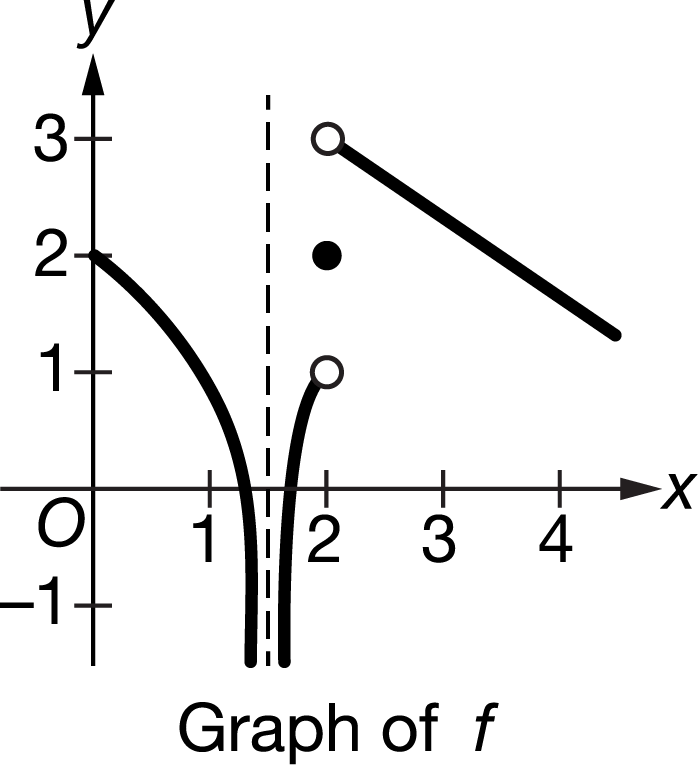
\includegraphics[scale=0.8]{vasymp1}
	\end{minipage}%
	\begin{minipage}{0.5\textwidth}
		\Large
		Find $\displaystyle\lim_{x\to1.5}f(x)$\\
		\\
		Find $\displaystyle\lim_{x\to0}f(x)$\\
		\\
		Find $\displaystyle\lim_{x\to2^{+}}f(x)$\\
		\\
		Find $\displaystyle\lim_{x\to4}f(x)$\\
	\end{minipage}\\
	\vspace*{\fill}
	\vspace*{\fill}
	\crono
	\resetcrono{\beamerbutton{reset}}
\end{frame}
\begin{frame}
	\frametitle{Exercise 1 - Solutions}
	\Large
	\[\displaystyle\lim_{x\to1.5}f(x) = -\infty\]\\
	\[\displaystyle\lim_{x\to0}f(x) = 0\]\\
	\[\displaystyle\lim_{x\to2^{+}}f(x) = 3\]\\
	\[\displaystyle\lim_{x\to4}f(x) = 1.5\]
\end{frame}
\begin{frame}
	\frametitle{Exercise 2}
	\initclock
	\vspace*{\fill}
	\vspace*{\fill}
	\vspace*{\fill}
	\initclock
	\begin{minipage}{0.6\textwidth}
		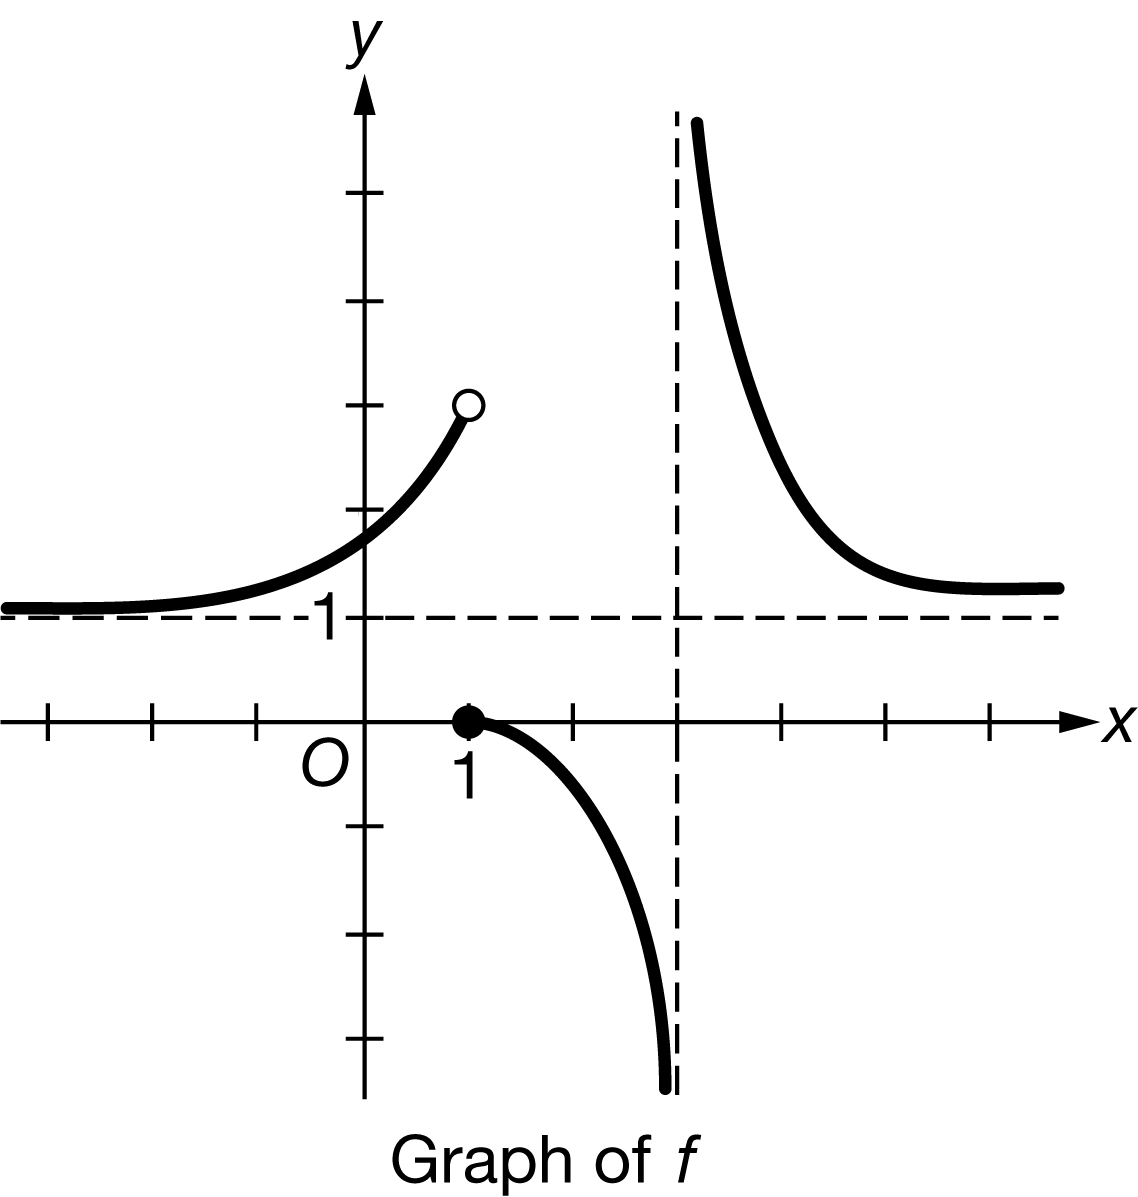
\includegraphics[scale=0.6]{vasymp2}
	\end{minipage}%
	\begin{minipage}{0.4\textwidth}
		\Large
		Find $\displaystyle\lim_{x\to1^{-}}f(x)$\\
		\\
		Find $\displaystyle\lim_{x\to1^{+}}f(x)$\\
		\\
		Find $\displaystyle\lim_{x\to3^{-}}f(x)$\\
		\\
		Find $\displaystyle\lim_{x\to3^{+}}f(x)$\\
	\end{minipage}\\
	\vspace*{\fill}
	\vspace*{\fill}
	\crono
	\resetcrono{\beamerbutton{reset}}
\end{frame}
\begin{frame}
	\frametitle{Exercise 2 - Solutions}
	\Large
	\[\displaystyle\lim_{x\to1^{-}}f(x) = 3\]\\
	\[\displaystyle\lim_{x\to1^{+}}f(x) = 0\]\\
	\[\displaystyle\lim_{x\to3^{-}}f(x) = -\infty\]\\
	\[\displaystyle\lim_{x\to3^{+}}f(x) = \infty\]
\end{frame}
\begin{frame}
	\frametitle{Exercise 3}
	\vspace*{\fill}
	\vspace*{\fill}
	\vspace*{\fill}
	\vspace*{\fill}
	\vspace*{\fill}
	\initclock
	\Large
	Find: \[\displaystyle\lim_{x\to2^{-}}\left(\frac{1-x^2}{x-2}\right) \text{ and } \displaystyle\lim_{x\to2^{+}}\left(\frac{1-x^2}{x-2}\right)\]\\
	\vspace*{\fill}
	\vspace*{\fill}
	\vspace*{\fill}
	\vspace*{\fill}
	\vspace*{\fill}
	\crono
	\resetcrono{\beamerbutton{reset}}
\end{frame}
\begin{frame}
	\frametitle{Exercise 3 - Solutions}
	\Large
	\[\displaystyle\lim_{x\to2^{-}}\left(\frac{1-x^2}{x-2}\right) = \infty\]\\
	\[\displaystyle\lim_{x\to2^{+}}\left(\frac{1-x^2}{x-2}\right) = -\infty\]
\end{frame}
\begin{frame}
	\frametitle{Exercise 4}
	\vspace*{\fill}
	\vspace*{\fill}
	\vspace*{\fill}
	\vspace*{\fill}
	\vspace*{\fill}
	\initclock
	\Large
	Find: \[\displaystyle\lim_{x\to1}\left[\frac{x-3}{(x-1)^2}\right]\]\\
	\vspace*{\fill}
	\vspace*{\fill}
	\vspace*{\fill}
	\vspace*{\fill}
	\vspace*{\fill}
	\crono
	\resetcrono{\beamerbutton{reset}}
\end{frame}
\begin{frame}
	\frametitle{Exercise 4 - Solutions}
	\Large
	\[\displaystyle\lim_{x\to1}\left[\frac{x-3}{(x-1)^2}\right] = -\infty\]
\end{frame}
\end{document}